\section{Signal and background modelling}
All samples, assuming $pp$ collisions at $\sqrt{s}=14$ \tev, are generated at LO in QCD using {\sc Madgraph5} 2.1.1 with the CTEQ6L1 PDF set, and interfaced with the {\sc Pythia} v6.427 parton shower and the Perugia2011C UE tune. The top-quark mass is set to 172 $\gev$ and top-quark decay is performed by {\sc Pythia}, as for $W/Z$-boson and Higgs-boson decays. 
  
\subsection{Signal modelling}

In this search the coupling of the CP-odd scalar (referred to as ``$A$ boson'') with the bottom and top quarks are added in the SM Lagrangian using a simplified-model approach:

\be
\mathcal{L}=\mathcal{L}_{\rm SM}+\mathcal{L}_{\rm CP-odd},
\ee

\noindent where

\be
\mathcal{L}_{CP-odd}=i\frac{g_{t}y_{t}}{\sqrt{2}}\bar{t}\gamma_{5}tA+i\frac{g_{b}y_{b}}{\sqrt{2}}\bar{b}\gamma_{5}bA,
\ee
 
\noindent and $g_{i}$ $(i=t,b)$ represents the deviation from the SM Yukawa coupling $y_{i}=m_{i}/v$. In this simplified approach, for $m_{b}<m_{A}<m_{t}$ the $A$ boson decays exclusively into bottom quarks with ${\rm BR}(A\to b\bar{b})=1$. The decay width, $\Gamma_{A}$, is determined by the value of $g_{b}$ and the event kinematic distributions, with assumption of a narrow width, do not depend on its value.
This model was implemented using {\sc FeynRules} 2.1 \cite{Alloul:2013bka} and imported as UFO model in {\sc Madgraph5}. Samples of $t\bar{t}A$ events were generated for different $A$-boson masses, $m_{A}$=20, 30, 40, 60, 80 and 100 $\gev$, assuming $g_{t}=1$. \par
A k-factor of 1.3,  obtained as the ratio of the NLO to LO cross sections for $t\bar{t}h$ production, where $h$ is a CP-even Higgs boson, is applied to the LO $t\bar{t}A$ signal cross section predicted by {\sc Madgraph5}. It has been checked that this k-factor is rather constant as a function of $m_{h}$, varied between 20 and 125 GeV.
The extra $\gamma_{5}$ factor present in the interaction between the CP-odd scalar and the top quark, compared to the case of a CP-even scalar, leads to two interesting features:

\bi
\ib a CP-odd scalar, at low mass, has harder $\pt$ spectrum compared to a CP-even scalar (see figure \ref{sec:ttA:fig:hpt}), and
\ib  the ratio $\sigma_{t\bar{t}h}/\sigma_{t\bar{t}A}$ varies significantly with mass, from about a factor of 20 at a mass of 20 $\gev$ to only about a factor of two at a mass of 120 $\gev$ (see figure \ref{sec:ttA:fig:xsec}).
\ei

\begin{figure}[htbp!]
\centering
\begin{subfigure}{0.45\textwidth}
  \centering
  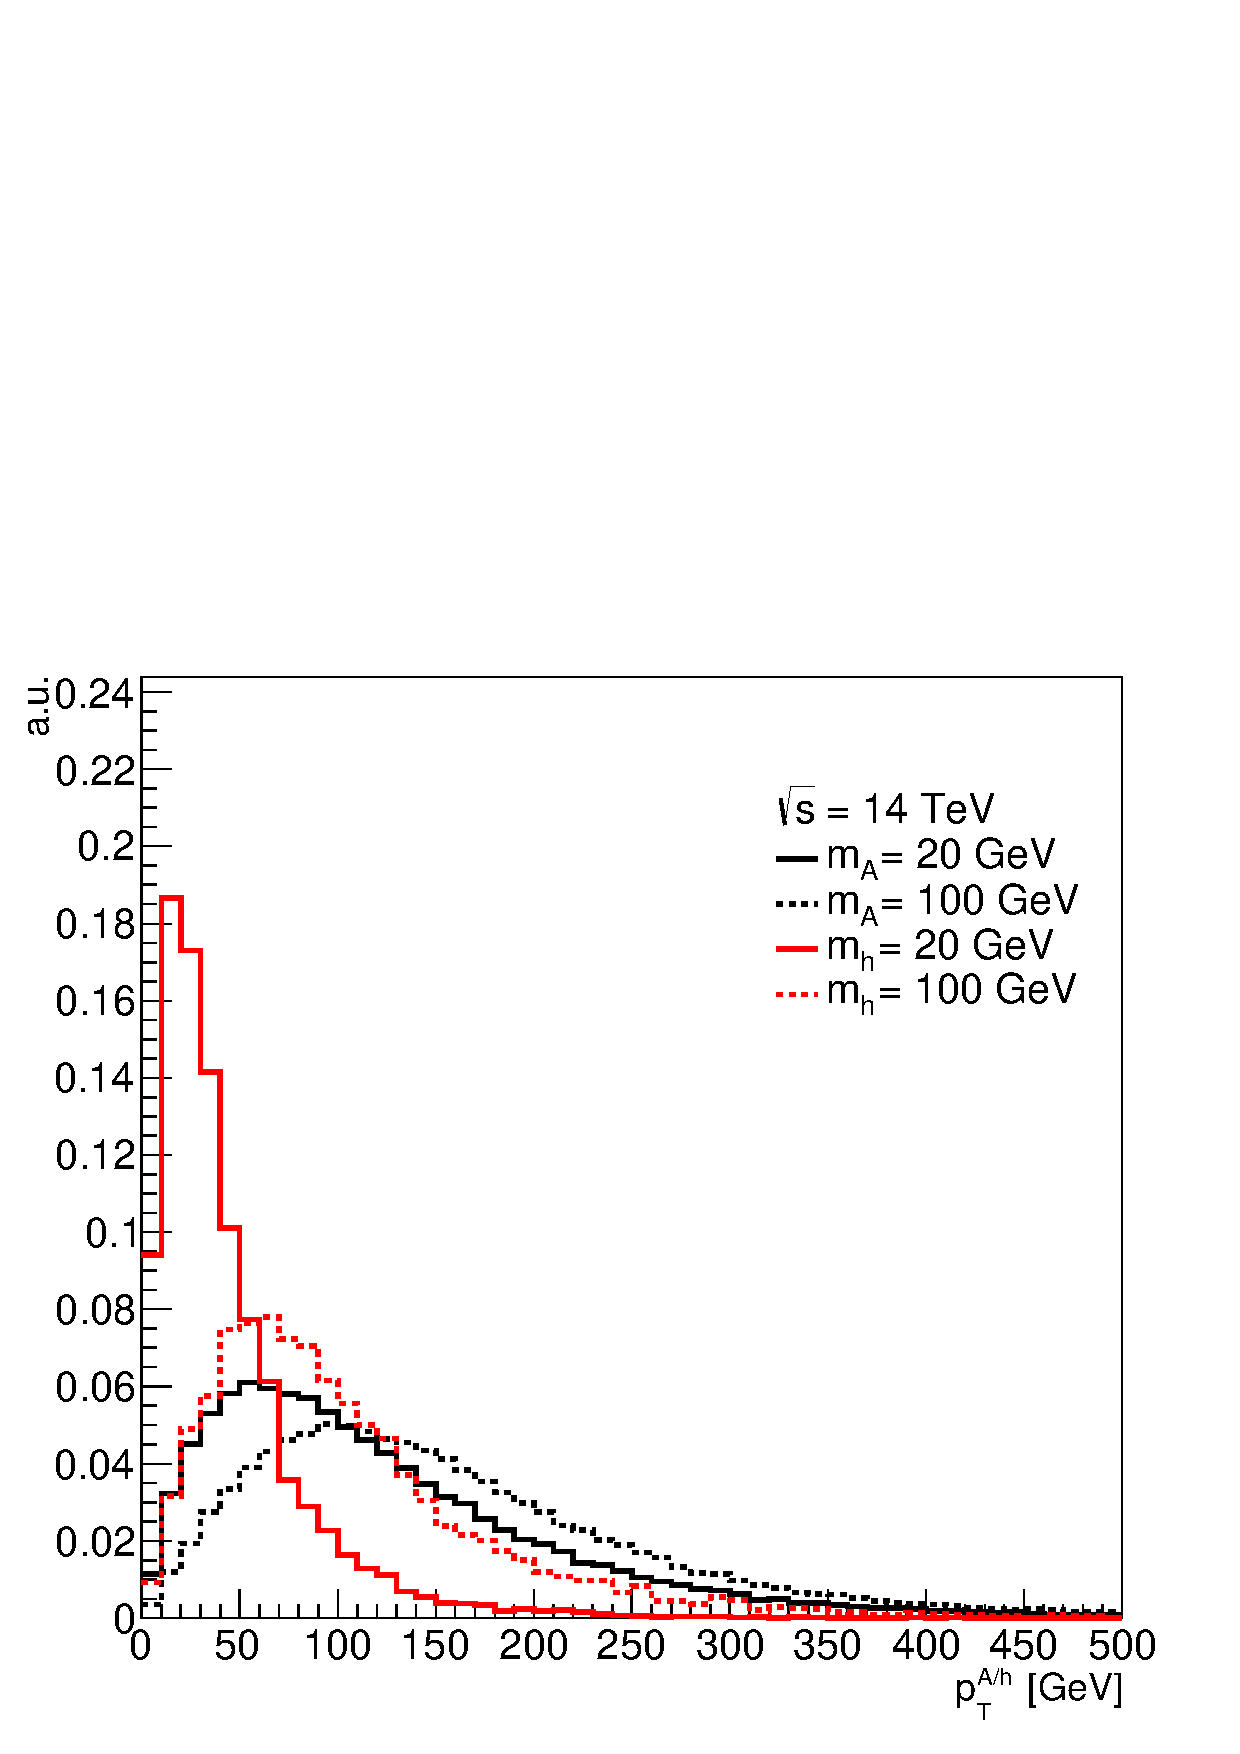
\includegraphics[width=0.9\textwidth]{figures/ttA/hpt.png}
  \caption{}
  \label{sec:ttA:fig:hpt}
\end{subfigure}
\begin{subfigure}{0.45\textwidth}
  \centering
  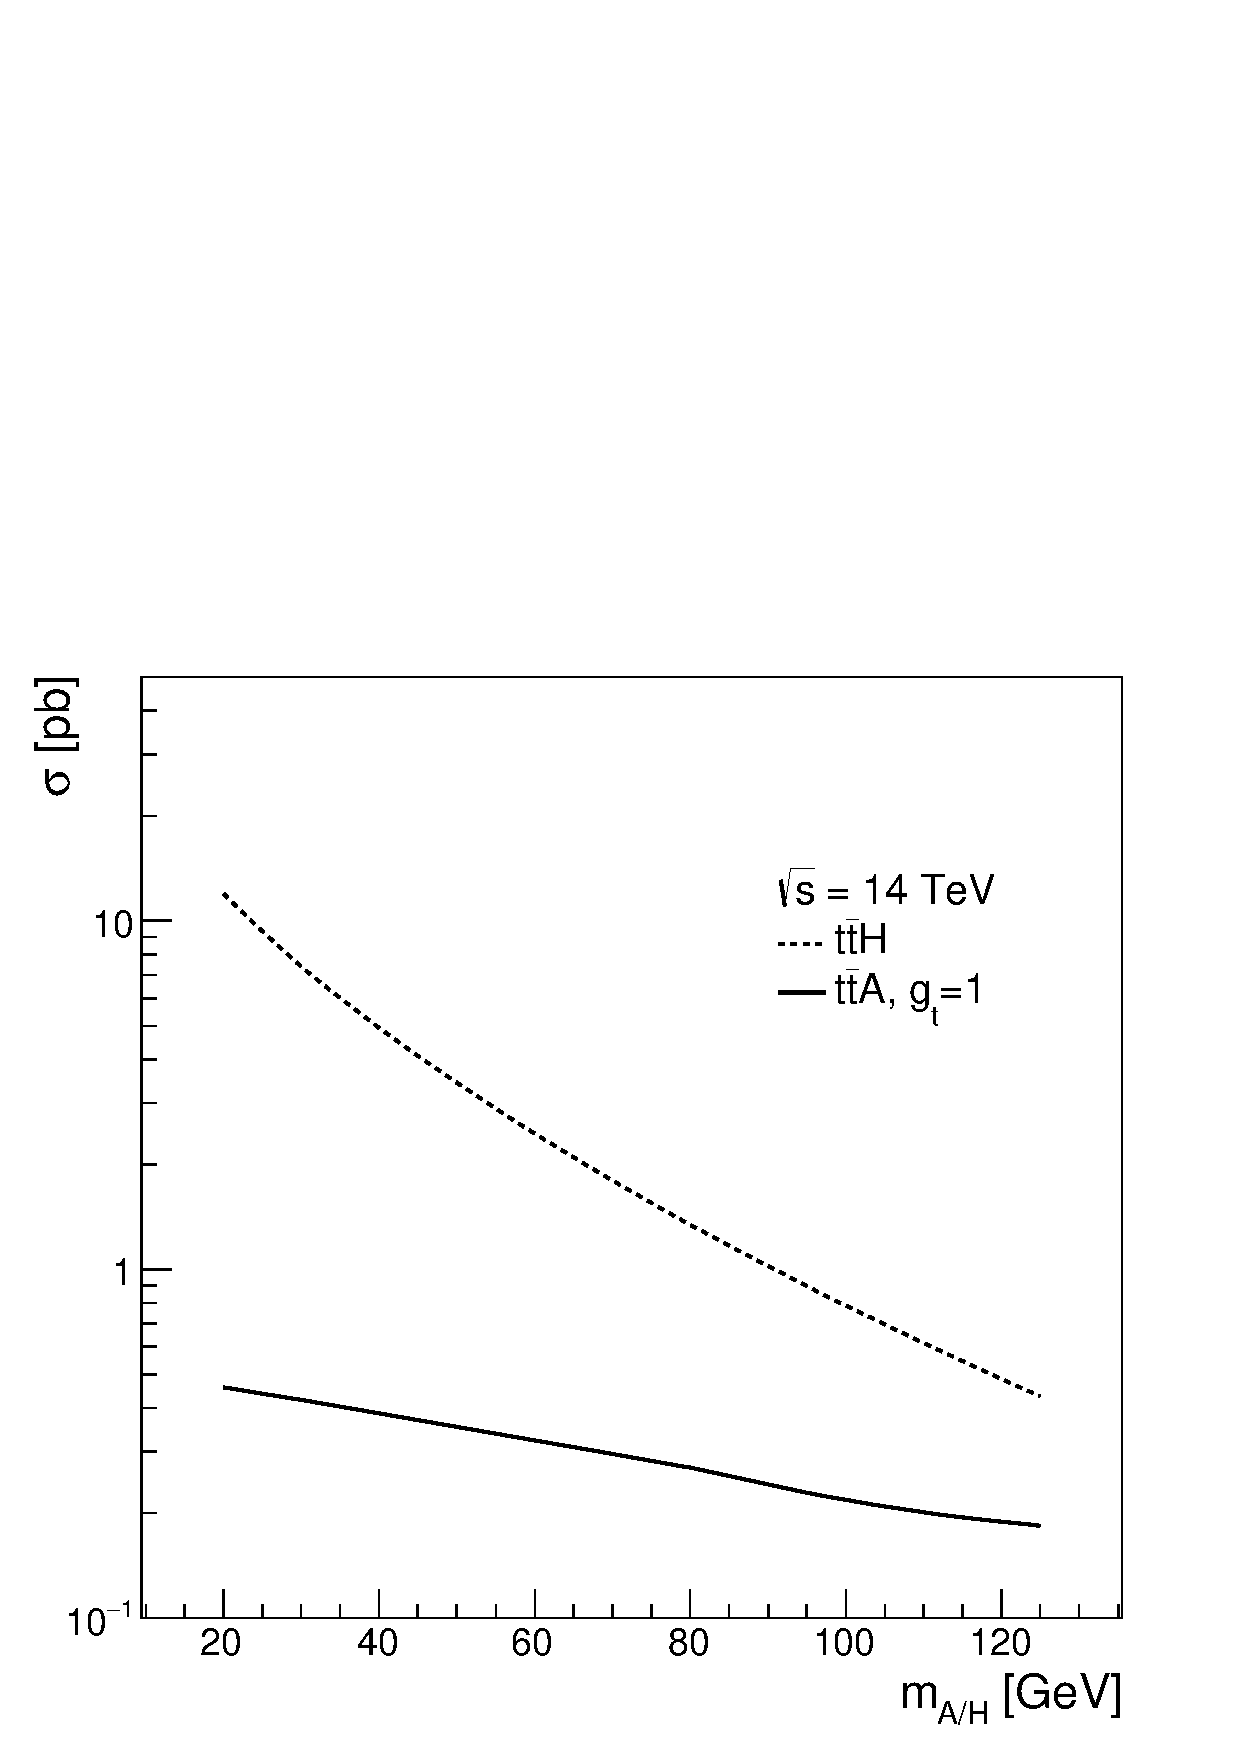
\includegraphics[width=0.9\textwidth]{figures/ttA/XSec.png}
  \caption{}
  \label{sec:ttA:fig:xsec}
\end{subfigure}
\captionsetup{width=0.85\textwidth} \caption{\small (a) Higgs-boson $\pt$ distribution for $t\bar{t}h$ (red) and $t\bar{t}A$ (black) for two different mass hypotheses: 20 $\gev$ (solid) and 100 $\gev$ (dashed). (b) Comparison of the LO cross section for $t\bar{t}h$ (solid line) and  $t\bar{t}A$ (dashed line) in $pp$ collisions at $\sqrt{s}$= 14 $\tev$ as a function of Higgs-boson mass.  In both cases a value of $g_{t}= 1$ is assumed.}
\label{sec:ttA:fig:gamma5}
\end{figure}


\subsection{Background modelling}

A sample of $t\bar{t}+$jets events is generated with up to two additional partons in the matrix element in the 5F scheme, and matched to the parton shower using the MLM prescription. 
The sample is normalised to to a cross section of 900 pb, computed at NNLO+NNLL cross section from {\sc TOP++} v2.0. The same procedure described in section \ref{chp:data:sec:ttbar} is used to categorise events according to the flavour content of extra jets in: $t\bar{t}+$light-jets, $t\bar{t}+\ge 1c$ and $t\bar{t}+\ge 1b$ (the latter two components together are usually referred as $t\bar{t}+$HF).

A sample of $t\bar{t}W$ events is generated requiring at least one $W$ boson in the event to decay leptonically, and  is  normalised  to  the  corresponding  LO  cross  section,  0.404  pb,  times  a  k-factor  of  1.4.\\
A sample of $t\bar{t}Z$ events is generated requiring $Z\to q\bar{q}$ decays and is normalised to the corresponding LO cross section,  0.353 pb,  times a
k-factor of 1.3. Finally, a sample of $t\bar{t}H$ events, with $H$ being the SM Higgs boson, is generated assuming $m_{H} = 125$ \gev and requiring $H\to b\bar{b}$ decays. It is normalised to the NLO cross section, 0.611 pb, times the $H\to b\bar{b}$ branching ratio of $57.7\%$. 

